\documentclass{beamer}
\usepackage[utf8]{inputenc}
\usepackage[T1]{fontenc}
\usepackage[english]{babel}
\usepackage{graphicx}
\usepackage{times}

\usetheme{AGH}

\title[Porównanie wydajności implementacji warstwy danych]{Porównanie wydajności rozwiązań implementujących warstwy dostępu do danych}

\author[K. Misiak]{Krzysztof Misiak}

\date[2017]{22.01.2011}

\institute[AGH-UST]
{Faculty of EEACSE\\ 
Department of Automatics
}

\setbeamertemplate{itemize item}{$\maltese$}

\begin{document}

{
% \usebackgroundtemplate{
\includegraphics[width=\paperwidth]{titlepage}} % wersja angielska
\usebackgroundtemplate{
\includegraphics[width=\paperwidth]{titlepagepl}} % wersja polska
 \begin{frame}
   \titlepage
 \end{frame}
}

%---------------------------------------------------------------------------


\begin{frame}
\frametitle{Ogólna architektura aplikacji}
\begin{center}
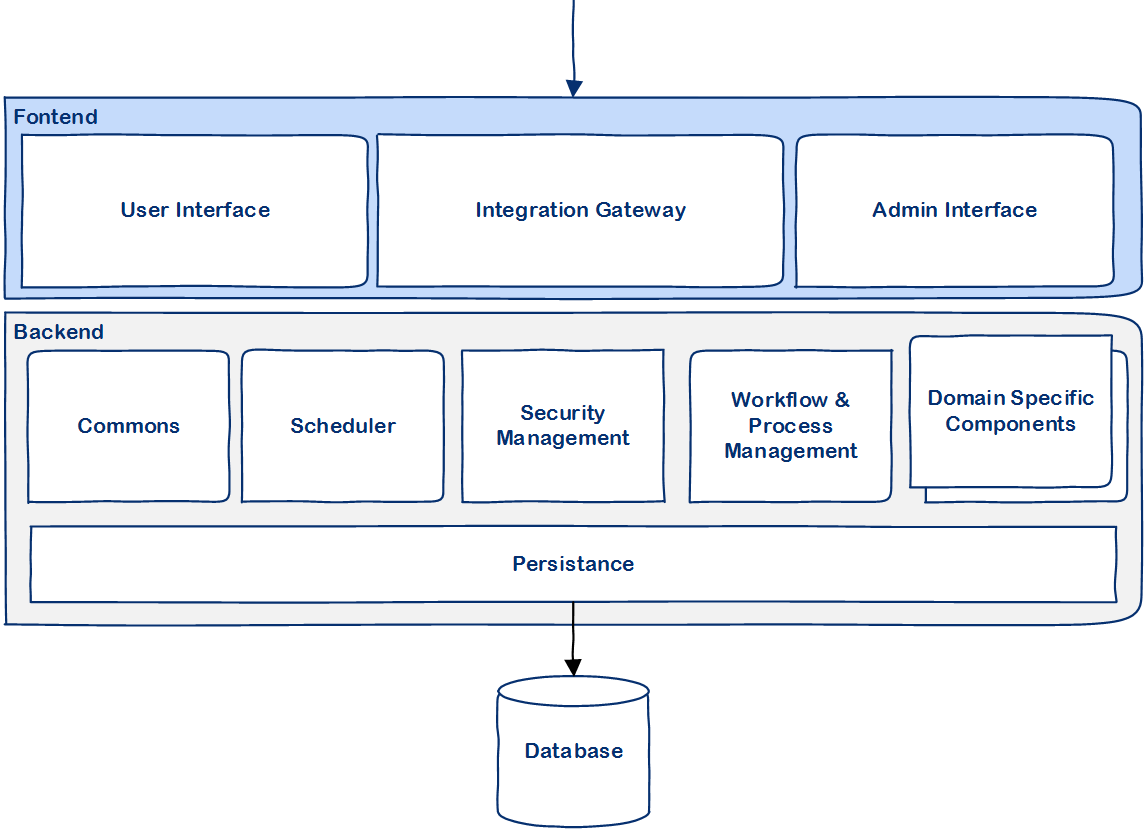
\includegraphics[height=.6\textheight,keepaspectratio]{architecture.png}
\end{center}
\end{frame}

\begin{frame}
\frametitle{Implementacje warstwy dostępu do danych}
\begin{itemize}
\item Mapowanie obiektowo-relacyjne ORM (Hibernate, PostgreSQL)
\item Bazy zorientowane dokumentowo (MongoDB)
\item System persystentny (Prevayler)
\end{itemize}
\end{frame}

\begin{frame}
\frametitle{Mapowanie obiektowo-relacyjne (ORM)}
\begin{itemize}
\item Sposób odwzorowania obiektowej architektury systemu informatycznego na relacyjną bazę danych
\item Rozwiązuje problem bezpośrednich odwołań do bazy przez wysoko-poziomowe funkcje
\item Łatwe do implementacji
\item Szybko może stać się wąskim gardłem bez odpowiednich optymalizacji
\end{itemize}
\end{frame}

\begin{frame}
\frametitle{Bazy zorientowane dokumentowo}
\begin{itemize}
\item Nie zawsze implementują wszystkie założenia ACID (Atomicity - atomowość, Consistency - spójność, Isolation - izolacja, Durability - trwałość)
\item Łatwo skalowalne, przeznaczone do przetwarzania bardzo dużych ilości danych
\item Nie ma wymagania jednorodności pod względem struktury
\end{itemize}
\end{frame}

\end{document}

